\documentclass[11pt,aspectratio=169]{beamer}

\usetheme{Madrid}
\usecolortheme{seahorse}

\usepackage[utf8]{inputenc}
\usepackage{amsmath,amssymb}
\usepackage{algpseudocode}
\usepackage{algorithmicx}
\usepackage{xcolor}
\usepackage{listings}
\usepackage{booktabs}
\usepackage{tikz}
\usetikzlibrary{arrows.meta,positioning,fit,backgrounds}

\setbeamertemplate{navigation symbols}{}
\setbeamertemplate{footline}[frame number]

\lstdefinestyle{py}{
  language=Python,
  basicstyle=\ttfamily\scriptsize,
  keywordstyle=\color{blue!70!black}\bfseries,
  commentstyle=\color{gray},
  stringstyle=\color{green!40!black},
  showstringspaces=false,
  breaklines=true,
  numbers=left,
  numberstyle=\tiny\color{gray},
  frame=single,
  xleftmargin=1.5em,
  aboveskip=0.3em,
  belowskip=0.3em
}

\title{LeetCode Deep Dive}
\subtitle{From First Instinct to Optimal Algorithm: Bipartite Coloring and Debt
Settlement in Practice\\
\small Week 11 Supplement -- TOAE209/TOAH209: Design and Analysis of Algorithms}
\author{Foreign Trade University}
\date{}

\begin{document}

% ---------------------------------------------------------------
\begin{frame}
  \titlepage
\end{frame}
% ---------------------------------------------------------------

\begin{frame}{Outline}
  \tableofcontents
\end{frame}

% =================================================================
\section{A Framework for Attacking a New Graph Problem}
% =================================================================

\begin{frame}{The four-step process, once more}
  \begin{enumerate}
    \item \textbf{First instinct.} Write the algorithm that follows most directly
    from re-reading the problem statement -- usually try-every-possibility.
    \item \textbf{Measure why it hurts.} Plug the actual constraints into the naive
    algorithm's complexity and watch it blow up.
    \item \textbf{Find the structural insight.} What property of the problem removes
    almost all of that wasted work?
    \item \textbf{Implement the optimal algorithm}, trace it by hand, then look for
    programming-level implementation tricks.
  \end{enumerate}
  \begin{alertblock}{This week's twist}
    Problem 1 (\emph{Is Graph Bipartite?}) gets a clean polynomial optimal algorithm --
    exactly the pattern from every previous week. Problem 2 (\emph{Optimal Account
    Balancing}) does \textbf{not}: it previews next week's topic, NP-completeness,
    where step 3 simply has no polynomial answer to find.
  \end{alertblock}
\end{frame}

% =================================================================
\section{Problem 1 (Medium): Is Graph Bipartite?}
% =================================================================

\begin{frame}{Problem statement}
  \begin{block}{LeetCode 785 -- Is Graph Bipartite? (\textcolor{blue!50!black}{Medium})}
    You are given an undirected graph on $n$ vertices $0,\dots,n-1$ as an adjacency
    list \texttt{graph} (no self-loops, no duplicate edges; possibly disconnected).
    Return \texttt{true} iff the vertices can be split into two sets so that every
    edge has one endpoint in each set.
  \end{block}
  \begin{itemize}
    \item Constraints (LeetCode): $1 \le n \le 100$.
    \item This is exactly this week's \textbf{bipartiteness} definition -- the same
    property that made the $s\to X\to Y\to t$ matching reduction well-defined in the
    first place.
  \end{itemize}
\end{frame}

\begin{frame}{Worked example}
  \begin{columns}
  \begin{column}{0.46\textwidth}
  \begin{center}
  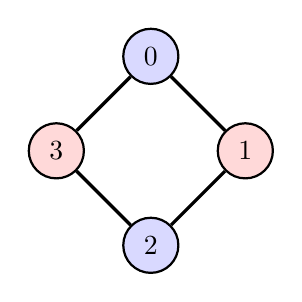
\begin{tikzpicture}[
      vtx/.style={circle, draw, thick, minimum size=7mm},
      >=Stealth]
    \node[vtx,fill=blue!15] (n0) at (0,1.2)   {0};
    \node[vtx,fill=red!15]  (n1) at (1.2,0)   {1};
    \node[vtx,fill=blue!15] (n2) at (0,-1.2)  {2};
    \node[vtx,fill=red!15]  (n3) at (-1.2,0)  {3};
    \draw[very thick] (n0)--(n1);
    \draw[very thick] (n1)--(n2);
    \draw[very thick] (n2)--(n3);
    \draw[very thick] (n3)--(n0);
  \end{tikzpicture}
  \end{center}
  \end{column}
  \begin{column}{0.54\textwidth}
  \small
  \texttt{graph = [[1,3],[0,2],[1,3],[0,2]]}
  \begin{itemize}
    \item A 4-cycle $0{-}1{-}2{-}3{-}0$: colors $\{0,2\}$ (blue) vs.\ $\{1,3\}$ (red) --
    every edge crosses colors. \textbf{Answer: true.}
    \item Contrast: a \emph{triangle} $0{-}1{-}2{-}0$ (odd cycle) can never be
    2-colored -- walking the cycle forces colors
    $A,B,A,\dots$ and an odd-length walk returns to a vertex demanding it be both $A$
    and $B$. \textbf{Answer: false.}
  \end{itemize}
  \end{column}
  \end{columns}
\end{frame}

\begin{frame}{First instinct: try every 2-coloring}
  \begin{block}{Most direct reading of the problem}
    ``Split vertices into two sets'' $\Rightarrow$ try every way of assigning each
    vertex to set $A$ or set $B$, and check whether \emph{some} assignment makes every
    edge cross sets.
  \end{block}
  \begin{algorithmic}[1]
    \For{each of the $2^n$ assignments $c: V \to \{A,B\}$}
      \If{every edge $(u,v)$ has $c(u) \neq c(v)$}
        \State \Return \textbf{true}
      \EndIf
    \EndFor
    \State \Return \textbf{false}
  \end{algorithmic}
\end{frame}

\begin{frame}{Why this is bad}
  \begin{itemize}
    \item Checking one assignment costs $O(E)$; there are $2^n$ assignments.
    \item Total: $O(2^n \cdot E)$. At the problem's own bound $n=100$: $2^{100}
    \approx 1.3\times10^{30}$ -- utterly impossible, even though $n=100$ is a tiny
    graph.
    \item The search treats each vertex's color as an \textbf{independent} choice.
    It is not: once one vertex's color is fixed, bipartiteness (if it holds at all)
    \textbf{forces} every neighbor's color.
  \end{itemize}
  \begin{alertblock}{The smell to notice}
    Whenever ``try all $2^n$ / $n!$ possibilities'' is the first instinct, ask: are
    these choices really independent, or does fixing one determine the rest?
  \end{alertblock}
\end{frame}

\begin{frame}{The structural insight}
  \begin{itemize}
    \item Within one connected component, pick any start vertex $s$ and color it $A$.
    Every neighbor of $s$ is then \textbf{forced} to $B$ (if the graph is bipartite at
    all); every neighbor of \emph{those} is forced back to $A$; and so on.
    \item So there is at most \textbf{one} candidate 2-coloring per component, not
    $2^n$ -- generate it by propagation (BFS/DFS), and check for a conflict (an edge
    whose two endpoints already share a color) \emph{as you go}.
    \item This is this week's own 2-coloring characterization of bipartiteness, run
    forward as an algorithm instead of used as a definition.
  \end{itemize}
\end{frame}

\begin{frame}{Optimal algorithm: BFS 2-coloring}
  \footnotesize
  \begin{algorithmic}[1]
    \Function{IsBipartite}{$G=(V,E)$}
      \State $color[v] \gets \text{None}$ for all $v$
      \For{each $s \in V$ with $color[s] = \text{None}$}
        \State $color[s] \gets A$;\ push $s$ onto queue $Q$
        \While{$Q$ not empty}
          \State $u \gets Q.\Call{pop}{}$
          \For{each neighbor $v$ of $u$}
            \If{$color[v] = \text{None}$}
              \State $color[v] \gets \text{opposite}(color[u])$;\ push $v$ onto $Q$
            \ElsIf{$color[v] = color[u]$}
              \State \Return \textbf{false} \Comment{conflict: same color, adjacent}
            \EndIf
          \EndFor
        \EndWhile
      \EndFor
      \State \Return \textbf{true}
    \EndFunction
  \end{algorithmic}
  One BFS pass per component, $O(V+E)$ total.
\end{frame}

\begin{frame}{Trace on the worked example}
  \small
  \texttt{graph = [[1,3],[0,2],[1,3],[0,2]]}, BFS from $0$.
  \begin{center}
  \begin{tabular}{@{}cllc@{}}
    \toprule
    step & action & queue after & conflict? \\
    \midrule
    1 & $color[0]\gets A$, push $0$ & $[0]$ & -- \\
    2 & pop $0$; neighbors $1,3$ uncolored $\to$ $color[1],color[3]\gets B$ & $[1,3]$
    & no \\
    3 & pop $1$; neighbor $0$ is $A\ (\neq B)$, ok; neighbor $2$ uncolored $\to A$ &
    $[3,2]$ & no \\
    4 & pop $3$; neighbor $0$ is $A\ (\neq B)$, ok; neighbor $2$ already $A\ (\neq B)$,
    ok & $[2]$ & no \\
    5 & pop $2$; neighbors $1,3$ both $B\ (\neq A)$, ok & $[]$ & no \\
    \bottomrule
  \end{tabular}
  \end{center}
  \begin{exampleblock}{Answer}
    No conflict found across the whole (single) component $\Rightarrow$
    \textbf{true}, coloring $\{0,2\}{=}A$, $\{1,3\}{=}B$ -- matches the diagram.
  \end{exampleblock}
\end{frame}

\begin{frame}{Complexity: naive vs.\ optimal}
  \begin{center}
  \begin{tabular}{@{}lll@{}}
    \toprule
    Approach & Time & At $n=100$ \\
    \midrule
    Try all $2^n$ colorings & $O(2^n E)$ & $\sim 10^{30}$ ops -- impossible \\
    \textbf{BFS/DFS propagation} & $\boldsymbol{O(V+E)}$ & $\le \sim 5000$ ops --
    instant \\
    \bottomrule
  \end{tabular}
  \end{center}
  The gap is not ``polynomial vs.\ slightly-worse polynomial'' -- it is
  ``polynomial vs.\ impossible,'' because the naive search never noticed that almost
  every one of its $2^n$ choices was already determined by an earlier one.
\end{frame}

\begin{frame}[fragile]{Python implementation}
  \begin{lstlisting}[style=py,aboveskip=0pt,belowskip=0pt]
from collections import deque

def isBipartite(graph):
    n = len(graph)
    color = [0] * n                 # 0 = uncolored, 1 / -1 = the two colors

    for start in range(n):
        if color[start] != 0:
            continue
        color[start] = 1
        queue = deque([start])
        while queue:
            u = queue.popleft()
            for v in graph[u]:
                if color[v] == 0:
                    color[v] = -color[u]        # forced to the opposite color
                    queue.append(v)
                elif color[v] == color[u]:
                    return False                 # same color, adjacent: conflict
    return True
  \end{lstlisting}
\end{frame}

\begin{frame}{Implementation tips \& tricks (the programming side)}
  \small
  \begin{itemize}
    \item \textbf{Encode colors as $\pm 1$, not strings/enums.} \texttt{-color[u]}
    flips the color in one machine op; comparing small integers is faster than
    comparing strings, and \texttt{0} doubles cleanly as the ``uncolored'' sentinel.
    \item \textbf{\texttt{deque.popleft()}, not \texttt{list.pop(0)}.} A plain Python
    list's \texttt{pop(0)} is $O(n)$ (it shifts every remaining element), silently
    turning a BFS you believe is $O(V+E)$ into $O(V^2)$ in practice.
    \item \textbf{Return \texttt{False} the instant a conflict appears.} Don't finish
    coloring the whole graph first and check afterward -- exiting early avoids wasted
    work exactly like Week 3's Union-Find returning at the first cycle-closing edge.
    \item \textbf{Loop over \emph{all} vertices as potential BFS starts.} The graph may
    be disconnected; forgetting the outer \texttt{for start in range(n)} loop silently
    ignores every component other than the first.
  \end{itemize}
\end{frame}

% =================================================================
\section{Problem 2 (Hard): Optimal Account Balancing}
% =================================================================

\begin{frame}{Problem statement}
  \begin{block}{LeetCode 465 -- Optimal Account Balancing (\textcolor{red!60!black}{Hard})}
    A list of transactions $[from_i, to_i, amount_i]$ records that person $from_i$
    gave person $to_i$ exactly $amount_i$ dollars. Return the \textbf{minimum number of
    transactions} required to settle all debts among the group.
  \end{block}
  \begin{itemize}
    \item Only each person's \textbf{net balance} matters -- who owes whom directly is
    irrelevant, only the final settlement count.
    \item This is a flow-\emph{shaped} problem (supplies and demands, like this week's
    circulations-with-demands), but the objective -- minimizing the transaction
    \textbf{count} -- is not one max-flow answers. Keep that tension in mind.
  \end{itemize}
\end{frame}

\begin{frame}{Worked example}
  \small
  \texttt{transactions = [[0,1,10],[2,0,5]]}
  \begin{center}
  \begin{tabular}{@{}lccc@{}}
    \toprule
    & person 0 & person 1 & person 2 \\
    \midrule
    after $[0,1,10]$ (0 pays 1) & $-10$ & $+10$ & $0$ \\
    after $[2,0,5]$ (2 pays 0) & $-10+5=-5$ & $+10$ & $-5$ \\
    \bottomrule
  \end{tabular}
  \end{center}
  Nonzero balances: $0:-5$, $1:+10$, $2:-5$.
  \begin{exampleblock}{A settlement in 2 transactions}
    $0$ pays $1$ exactly \$5 (zeroes out $0$, leaves $1$ at $+5$); $2$ pays $1$ exactly
    \$5 (zeroes out both). \textbf{Answer: 2} -- matches LeetCode's own Example 1.
  \end{exampleblock}
\end{frame}

\begin{frame}{First instinct: try every settlement order}
  \begin{block}{Most direct reading of the problem}
    ``Find the minimum number of transactions'' $\Rightarrow$ try every way of pairing
    up nonzero balances and transferring money between them, and take the best.
  \end{block}
  \begin{itemize}
    \item Naively: at each step, pick \emph{any} two nonzero balances of opposite sign
    and transfer the smaller amount between them; branch over \textbf{every} such pair,
    recurse, count transactions, minimize over all branches.
    \item With $k$ nonzero balances, the number of distinct ways to fully pair/group
    them grows combinatorially -- for $k=12$, well past $10^8$ branches with no
    pruning.
  \end{itemize}
\end{frame}

\begin{frame}{Why this is bad}
  \begin{itemize}
    \item Unlike Problem 1, there is \textbf{no known polynomial algorithm} for this
    objective: deciding whether $k$ nonzero balances can be settled in exactly
    $k - g$ transactions (for $g$ independent zero-sum groups) is equivalent to
    partitioning a multiset into zero-sum subsets -- a problem in the same
    NP-hard family as \emph{Partition} and \emph{Subset Sum}.
    \item So ``why is this bad'' is not just ``the constant is too big'' -- it is
    ``no algorithm known to anyone runs in polynomial time on this exact objective.''
    This is next week's topic previewed early.
  \end{itemize}
  \begin{alertblock}{The honest complexity story}
    LeetCode bounds \texttt{transactions.length} $\le 8$, so at most $16$ people and
    usually far fewer nonzero balances after netting -- small enough that a
    well-pruned exponential search is fast in practice, even though no polynomial
    algorithm exists.
  \end{alertblock}
\end{frame}

\begin{frame}{The structural insight (pruning, not a polynomial bound)}
  \begin{itemize}
    \item \textbf{WLOG reduction:} in \emph{some} optimal solution, the person holding
    the \emph{first} nonzero balance transacts with one specific other person. So at
    each recursion level, only try pairing balance[0] with each of the other nonzero
    balances -- branching factor $k-1$ instead of an unstructured search over all
    pairings.
    \item \textbf{Free pruning:} if balance[0] happens to already be $0$ (because an
    earlier transfer zeroed it exactly), skip straight to the next nonzero balance
    \emph{without} counting a transaction -- this automatically detects and exploits
    any zero-sum subgroup that can settle independently.
    \item Still exponential worst case -- but these two rules are exactly what makes
    the search fast enough for LeetCode's $k \le 16$.
  \end{itemize}
\end{frame}

\begin{frame}{Optimal (best-known) algorithm: pruned backtracking}
  \footnotesize
  \begin{algorithmic}[1]
    \Function{Settle}{$balances[\,]$}
      \State skip leading zero entries (advance index $i$ while $balances[i]=0$)
      \If{$i \geq$ length of $balances$} \Return $0$ \EndIf
      \State $best \gets \infty$
      \For{each $j > i$ with $balances[j]$ opposite sign to $balances[i]$}
        \State $balances[j] \gets balances[j] + balances[i]$;\ save old $balances[i]$
        \State $balances[i] \gets 0$
        \State $best \gets \min(best,\ 1 + \Call{Settle}{balances[\,]})$
        \State undo: restore $balances[i]$ and $balances[j]$
      \EndFor
      \State \Return $best$
    \EndFunction
  \end{algorithmic}
  Exponential worst case; fast in practice because of the pruning above.
\end{frame}

\begin{frame}{Trace on the worked example}
  \small
  Nonzero balances (order found): $[-5, +10, -5]$ (person $0$, $1$, $2$).
  \begin{center}
  \begin{tabular}{@{}cll@{}}
    \toprule
    call & state & choice \\
    \midrule
    \textsc{Settle}$([-5,10,-5])$ & $i=0$, $balances[0]=-5$ & try $j=1$: $10-5=5$
    $\to [0,5,-5]$ \\
    \textsc{Settle}$([0,5,-5])$ & $i=1$ ($balances[0]$ now $0$, skip free) &
    try $j=2$: $-5+5=0 \to [0,0,0]$ \\
    \textsc{Settle}$([0,0,0])$ & all zero & \Return $0$ \\
    \bottomrule
  \end{tabular}
  \end{center}
  \begin{exampleblock}{Answer}
    Unwinding: $1 + (1 + 0) = 2$ transactions -- $0\to1$ (\$5), $2\to1$ (\$5). Matches
    the hand-computed answer.
  \end{exampleblock}
\end{frame}

\begin{frame}[fragile]{Python implementation (part 1: net balances)}
  \begin{lstlisting}[style=py,aboveskip=0pt,belowskip=0pt]
def minTransfers(transactions):
    net = {}
    for u, v, amount in transactions:
        net[u] = net.get(u, 0) - amount
        net[v] = net.get(v, 0) + amount
    balances = [b for b in net.values() if b != 0]
    # settle(...) is defined next, then called as: return settle(0)
  \end{lstlisting}
  Only \emph{nonzero} net balances ever enter the search -- everyone else is already
  settled and contributes zero transactions.
\end{frame}

\begin{frame}[fragile]{Python implementation (part 2: pruned backtracking)}
  \begin{lstlisting}[style=py,aboveskip=0pt,belowskip=0pt]
    def settle(i):
        while i < len(balances) and balances[i] == 0:
            i += 1                              # free: already-zero prefix
        if i == len(balances):
            return 0
        best = float('inf')
        for j in range(i + 1, len(balances)):
            if balances[j] * balances[i] < 0:   # opposite signs only
                balances[j] += balances[i]
                old = balances[i]
                balances[i] = 0
                best = min(best, 1 + settle(i + 1))
                balances[i] = old
                balances[j] -= balances[i]
        return best

    return settle(0)
  \end{lstlisting}
\end{frame}

\begin{frame}{Implementation tips \& tricks (the programming side)}
  \small
  \begin{itemize}
    \item \textbf{Work in integer cents, not float dollars.} Summing floating-point
    amounts can leave a balance at \texttt{-4.999999999} instead of exactly \texttt{-5},
    so the ``skip if balance == 0'' pruning silently breaks. LeetCode's inputs are
    integers -- keep every intermediate value an \texttt{int}.
    \item \textbf{Filter zero balances \emph{before} recursing.} Building
    \texttt{balances} only from \texttt{net.values() if b != 0} shrinks the search
    space immediately -- people who already balance out never enter the backtracking
    at all.
    \item \textbf{Mutate-and-undo beats copying the list.} Restoring
    \texttt{balances[i]}/\texttt{balances[j]} after the recursive call avoids allocating
    a new list at every one of the (many) recursive calls -- a real constant-factor
    win when the search tree is already exponential.
  \end{itemize}
\end{frame}

% =================================================================
\section{Summary}
% =================================================================

\begin{frame}{Summary: two problems, one contrast}
  \footnotesize
  \begin{enumerate}
    \item \textbf{Is Graph Bipartite?} follows this course's usual arc: a naive
    $2^n$ search turns out to be full of redundant, forced choices, and exploiting
    that gives a clean $O(V+E)$ polynomial algorithm -- BFS 2-coloring, the same idea
    underlying this week's matching reduction.
    \item \textbf{Optimal Account Balancing} breaks that arc on purpose: minimizing the
    transaction \emph{count} is equivalent to a zero-sum partitioning problem with no
    known polynomial algorithm. The best we can do is prune an exponential search
    (WLOG pairing + free zero-skipping) and rely on the input being small.
    \item That contrast \emph{is} the lesson: flow-shaped problems are not
    automatically easy -- max-flow makes \emph{matching size} and \emph{cut value}
    easy, but a different objective on the same kind of data (transaction
    \emph{count}) can land you in NP-hard territory instead.
  \end{enumerate}
  \begin{alertblock}{Keep practicing}
    \texttt{LEETCODE.md} lists four more Week 11 problems (\emph{Possible
    Bipartition}, \emph{Maximum Number of Accepted Invitations}, \emph{Minimum Number
    of Vertices to Reach All Nodes}, \emph{Course Schedule II}) -- and next week's
    Intractability lecture will explain \emph{why} Problem 2 above resisted a clean
    polynomial algorithm.
  \end{alertblock}
\end{frame}

\end{document}
